\newpage
\section{Klasyfikacja informacji publikowanych w\,social media}
W poniższym rozdziale opisano przebieg i\,wyniki klasyfikacji postów pobranych z\,Twee- tera pod względem przynależności do jednej z\,dwóch klas. Badania te oparto na pracy Some Like it Hoax\cite{tacchini2017some} w\,której przeprowadzono klasyfikację postów pobranych z\,platformy facebook otrzymawszy bardzo wysoką precyzję. Celem badań w\,obecnej pracy jest sprawdzenie możliwości klasyfikacji postów z\,zebranego zbioru polskojęzycznego. Klasyfikacja będzie dokonywana na podstawie informacji o\,udostępnieniach tych postów przez użytkowników. Dodatkowym celem jest sprawdzenie jak duży musi być zbiór zaklasyfikowanych danych podany jako zbiór uczący, aby otrzymać zadowalającą precyzję klasyfikacji.
\subsection{Opis badań Some Like It Hoax}
Badania w\,pracy Some Like it Hoax opierano na postach publikowanych przez wybrane konta na platformie Facebook. Konta te były zaklasyfikowane do odpowiedniej z\,dwóch klas. Dla wszystkich postów pobrano również informacje, o\,osobach które ten post polubiły. Używając tych danych przeprowadzono klasyfikację przy pomocy algorytmu regresji logistycznej oraz autorskiej modyfikacji algorytmu traktując problem tej klasyfikacji jak problem binarnego etykietowania poprzez crowsourcing (eng. boolean label crowdsourcing).
Wykorzystując fakt, że większość użytkowników ograniczała swoją aktywność tyko do postów należących do tylko jednej z\,tych kategorii, ale istnieje też niemała grupa akceptująca oba rodzaje stron możliwe było osiągnięcie bardzo wysokich wyników klasyfikacji postów do odpowiedniej kategorii. Jednak również wykorzystując grupy użytkowników niespolaryzowanych możliwe było rozpoznanie klasy posta z\,wysokim prawdopodobieństwem.
\subsubsection{Opis wyników badań}
Do badań w\,2017 roku pobrano 15,500 postów polubionych 2 miliony razy przez ponad 900 tysięcy użytkowników. Dla obu użytych algorytmów przeprowadzano badania dla dwóch zbiorów danych z\,różniącymi się wskaźnikami. Były nimi zbiór wszystkich postów wraz ze wszystkimi użytkownikami. Oraz zbiór postów polubionych przez użytkowników, którzy polubili posty z\,obu klas nazwany zbiorem intersekcji. W\,trakcie badań udało się twórcom uzyskać bardzo wysokie wyniki. 
\par
Najwyższe wyniki uzyskano dla algorytmu harmonicznego traktującego cały zbiór danych jako zmodyfikowany problem etykietowania. Dla takiego zestawienia uzyskiwano prawie perfekcyjną dokładność 99,4\% nawet gdy w\,zbiorze trenującym znajdowało się 0,5\% danych, czyli 80postów
W przypadku tylko zbioru intersekcji nieznacznie lepsza okazała się być metoda regresji logistycznej. Uzyskano precyzję na poziomie 90\% przy wykorzystaniu 10\% zbioru do nauki modelu. 
\par 
Poniżej na rysunku \ref{fig:wyniki-somelikeithoax} załączono wykres prezentujący całościowe wyniki tej pracy. Przedstawia on wyniki precyzji na osi y względem wielkości zbioru uczącego wyrażonego w jego stosunku do wielkości całego zbioru. Na tym wykresie pokazano cztery serie danych po dwie dla każdego z zbiorów danych dla każdego z algorytmów: regresji logistycznej oraz algorytmu harmonicznego.

\begin{figure}[!h]
	
	\centering 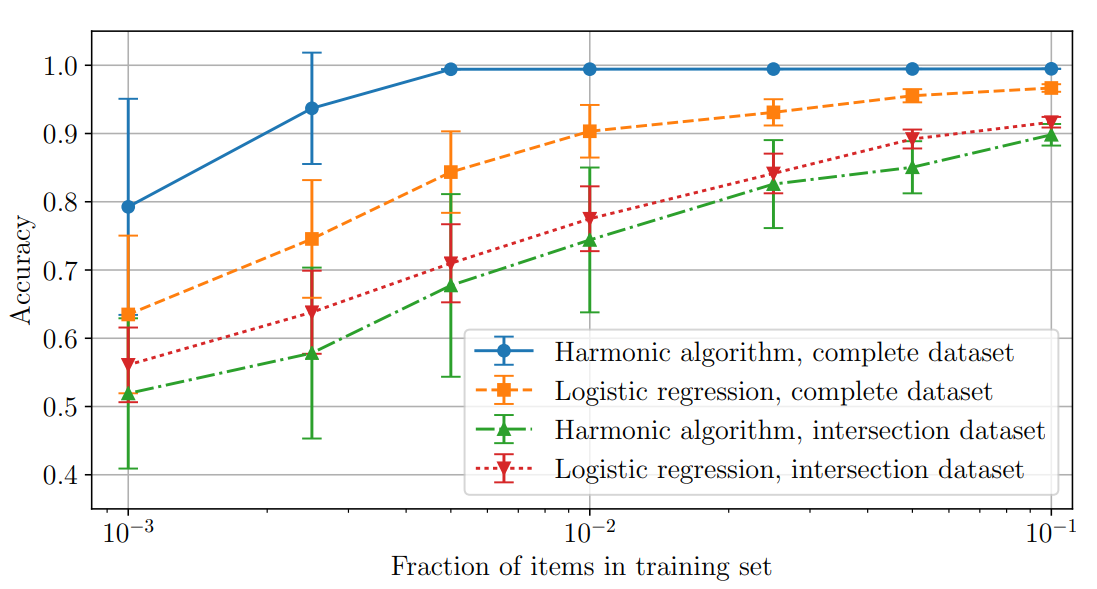
\includegraphics[width=0.9\linewidth]{img/results/wyniki-somelikeithoax.png}
	\caption{Wyniki badań klasyfikacji postów pochodzących z platformy Facebook. Źródło:\cite{tacchini2017some}}\label{fig:wyniki-somelikeithoax}
\end{figure}
